\apendice{Especificación de Requisitos}

\section{Introducción}
Este apartado de los anexos contempla la especificación de los requisitos del proyecto desarrollado. Este apartado es de gran importancia debido a su utilidad para dejar unas pautas claras acerca de qué funcionalidades se esperan y para definir una buena planificación de tareas que asegure un desarrollo satisfactorio del proyecto.

\section{Objetivos generales}
Este proyecto tiene como objetivos principales los siguientes:
\begin{itemize}
    \item Proporcionar una herramienta web que ofrezca un catálogo de libros de prehistoria aptos para la infancia en base a los hallazgos científicos respecto a los roles de género, y mejorar así la educación o al menos asegurar que no se perpetúan los sesgos de género que ya han sido clarificados por la ciencia.
    \item Aportar una  herramienta didáctica para que cualquier persona pueda evaluar la adecuación de un libro, mostrando para ello la metodología de evaluación seguida en el catálogo. 
    \item Brindar herramientas al personal de gestión del catálogo para poder modificar los datos internos de la aplicación mediante una interfaz gráfica.
    \item Almacenar los libros mostrados de manera segura con opciones de carga y descarga de los datos.
\end{itemize}

\section{Catálogo de requisitos}
En este apartado se muestran todos los requisitos funcionales y no funcionales recogidos en el proyecto.

\subsection{Requisitos Funcionales}

\begin{enumerate}
    \item \textbf{RF-1: Gestión de catálogo}
    \begin{enumerate}
        \item \textbf{RF-1.1: Listar libros} Permitir a la persona con rol de administración ver una lista completa de libros disponibles.
        \item \textbf{RF-1.2: Editar libro} Permitir a la persona con rol de administración modificar la información de un libro existente.
        \item \textbf{RF-1.3: Eliminar libro} Permitir a la persona con rol de administración borrar un libro del catálogo.
        \item \textbf{RF-1.4: Selección de libro} Permitir a la persona con rol de administración seleccionar libros específicos.
    \end{enumerate}

    \item \textbf{RF-2: Agregar libro manual}
    \begin{enumerate}
        \item \textbf{RF-2.1:} Permitir a la persona con rol de administración agregar nuevos libros al catálogo de forma manual.
    \end{enumerate}

    \item \textbf{RF-3: Agregar libro automático}
    \begin{enumerate}
        \item \textbf{RF-3.1: Agregar libro automático} Permitir a la persona con rol de administración agregar libros al catálogo de forma automática desde diversas fuentes.
        \item \textbf{RF-3.2: Combinar fuentes} Unificar datos de libros provenientes de diferentes fuentes y guardarlo como uno.
    \end{enumerate}

    \item \textbf{RF-4: Gestión de roles}
    \begin{enumerate}
        \item \textbf{RF-4.1: Crear rol} Permitir a la persona con rol de administración definir nuevos roles de usuario.
        \item \textbf{RF-4.2: Editar rol} Permitir a la persona con rol de administración modificar roles existentes.
        \item \textbf{RF-4.3: Eliminar rol} Permitir a la persona con rol de administración eliminar roles.
        \item \textbf{RF-4.4: Listar roles} Mostrar una lista de roles disponibles.
        \item \textbf{RF-4.5: Gestionar permisos} Asignar permisos específicos a los roles.
    \end{enumerate}

    \item \textbf{RF-5: Gestión de usuarios}
    \begin{enumerate}
        \item \textbf{RF-5.1: Crear usuario} Permitir a la persona con rol de administración agregar nuevos usuarios al sistema.
        \item \textbf{RF-5.2: Editar usuario} Permitir a la persona con rol de administración modificar la información de usuarios existentes.
        \item \textbf{RF-5.3: Eliminar usuario} Permitir a la persona con rol de administración borrar usuarios.
        \item \textbf{RF-5.4: Listar usuarios} Mostrar una lista de usuarios registrados en el sistema.
        \begin{enumerate}
        \item \textbf{RF-5.5: Cambiar contraseña} Permitir a los usuarios registrados cambiar su contraseña.
    \end{enumerate}
    \end{enumerate}

    \item \textbf{RF-6: Importar catálogo}
    \begin{enumerate}
        \item \textbf{RF-6.1:} Permitir a la persona con rol de administración importar un catálogo de libros desde un archivo externo.
    \end{enumerate}

    \item \textbf{RF-7: Exportar catálogo}
    \begin{enumerate}
        \item \textbf{RF-7.1:} Permitir a la persona con rol de administración exportar el catálogo de libros a un archivo.
    \end{enumerate}

    \item \textbf{RF-8: Gestionar actividades incluidas en la evaluación de libros}
    \begin{enumerate}
        \item \textbf{RF-8.1: Crear actividad} Permitir a la persona con rol de administración definir nuevas actividades.
        \item \textbf{RF-8.2: Editar actividad} Permitir a la persona con rol de administración modificar actividades existentes.
        \item \textbf{RF-8.3: Eliminar actividad} Permitir a la persona con rol de administración borrar actividades.
        \item \textbf{RF-8.4: Listar actividades} Mostrar una lista de actividades disponibles.
        \item \textbf{RF-8.5: Obtener actividades} Obtener actividades disponibles del \textit{backend}.
    \end{enumerate}

    \item \textbf{RF-9: Iniciar sesión}
    \begin{enumerate}
        \item \textbf{RF-9.1:} Permitir a los usuarios autenticarse en el sistema para acceder a sus funcionalidades.
    \end{enumerate}

    \item \textbf{RF-10: Buscar libro}
    \begin{enumerate}
        \item \textbf{RF-10.1:} Permitir a los usuarios buscar libros específicos en el catálogo.
    \end{enumerate}

    \item \textbf{RF-11: Obtener catálogo}
    \begin{enumerate}
        \item \textbf{RF-11.1:} Permitir a los usuarios obtener el catálogo completo de libros.
    \end{enumerate}

    \item \textbf{RF-12: Obtener información de libro}
    \begin{enumerate}
        \item \textbf{RF-12.1:} Permitir a los usuarios ver la información detallada de un libro específico.
    \end{enumerate}
    
    \item \textbf{RF-13: Gestionar valoraciones}
    \begin{enumerate}
        \item \textbf{RF-13.1: Eliminar valoraciones} Permitir a los responsables de la administración eliminar valoraciones.
        \item \textbf{RF-13.2: Listar valoraciones} Mostrar una lista de valoraciones realizadas por los usuarios.
    \end{enumerate}

    \item \textbf{RF-14: Obtener estadísticas}
    \begin{enumerate}
        \item \textbf{RF-14.1:} Realizar los cálculos necesarios y obtener las estadísticas guardadas en base de datos y mostrarlo
    \end{enumerate}

    \item \textbf{RF-15: Generar valoraciones}
    \begin{enumerate}
        \item \textbf{RF-15.1:} Permitir la generación de valoraciones basadas en parámetros definidos.
    \end{enumerate}

    \item \textbf{RF-16: Crear sugerencia}
    \begin{enumerate}
        \item \textbf{RF-16.1:} Permitir a los usuarios enviar sugerencias sobre libros.
    \end{enumerate}
    
\end{enumerate}

\subsection{Requisitos No Funcionales}

\begin{enumerate}
    \item \textbf{RNF-1: Seguridad}
    \begin{enumerate}
        \item \textbf{RNF-1.1:} Implementar autenticación y autorización mediante JWT para proteger el acceso a la API.
        \item \textbf{RNF-1.2:} Asegurar que los datos personales de los usuarios estén encriptados y protegidos contra accesos no autorizados.
    \end{enumerate}

    \item \textbf{RNF-2: Rendimiento}
    \begin{enumerate}
        \item \textbf{RNF-2.1:} La aplicación debe ser capaz de manejar un gran número de solicitudes simultáneas sin degradar su rendimiento.
        \item \textbf{RNF-2.2:} Optimizar las consultas a la base de datos para asegurar tiempos de respuesta rápidos.
    \end{enumerate}

    \item \textbf{RNF-3: Usabilidad}
    \begin{enumerate}
        \item \textbf{RNF-3.1:} La interfaz de usuario debe ser intuitiva y fácil de usar para asegurar una experiencia agradable.
        \item \textbf{RNF-3.2:} El diseño debe ser adaptativo para asegurar que la interfaz se vea y funcione correctamente en distintos dispositivos y tamaños de pantalla.
    \end{enumerate}

    \item \textbf{RNF-4: Escalabilidad}
    \begin{enumerate}
        \item \textbf{RNF-4.1:} El sistema debe ser escalable para poder manejar un creciente número de usuarios y datos.
        \item \textbf{RNF-4.2:} El sistema debe ser escalable en términos funcionales, permitiendo la adición de nuevas funcionalidades sin comprometer el rendimiento.
    \end{enumerate}

    \item \textbf{RNF-5: Compatibilidad}
    \begin{enumerate}
        \item \textbf{RNF-5.1:} La aplicación debe ser compatible con los principales navegadores web.
        \item \textbf{RNF-5.2:} Asegurar que la aplicación funcione correctamente en diferentes dispositivos, incluyendo móviles y tablets.
    \end{enumerate}

    \item \textbf{RNF-6: Mantenimiento}
    \begin{enumerate}
        \item \textbf{RNF-6.1:} El código debe estar bien documentado y estructurado para facilitar su mantenimiento y actualización.
    \end{enumerate}

    \item \textbf{RNF-7: Disponibilidad}
    \begin{enumerate}
        \item \textbf{RNF-7.1:} La aplicación debe estar disponible el 99.9\% del tiempo, asegurando un mínimo de tiempo de inactividad.
        \item \textbf{RNF-7.2:} Implementar estrategias de backup y recuperación para asegurar la disponibilidad de los datos en caso de fallos.
    \end{enumerate}
\end{enumerate}

\section{Especificación de requisitos}
Antes de comenzar con los casos de uso, se muestra el diagrama para un entendimiento rápido y visual. Debido a la complejidad y al gran número de funcionalidades, se han separado en dos diagramas para su mejor comprensión. 

La figura \ref{Diagrama conexión de funciones con autenticación} representa el conjunto de todas las zonas restringidas de la aplicación que contienen un lazo de dependencia con la funcionalidad de iniciar sesión.

La figura \ref{Diagrama de casos de uso} muestra un diagrama de casos de uso tradicional en el que se cuenta con dos roles, un administrador que tiene acceso a todas las funcionalidades y un usuario que solo puede acceder a elementos limitados.

\begin{figure}[htbp]
    \centering
    \includegraphics[width=1\linewidth]{Imagenes/Diagrama de casos de uso-Página-2.drawio.png}
    \caption{Diagrama conexión de funciones con autenticación}
    \label{Diagrama conexión de funciones con autenticación}
\end{figure}
\FloatBarrier

\begin{figure}[htbp]
    \centering
    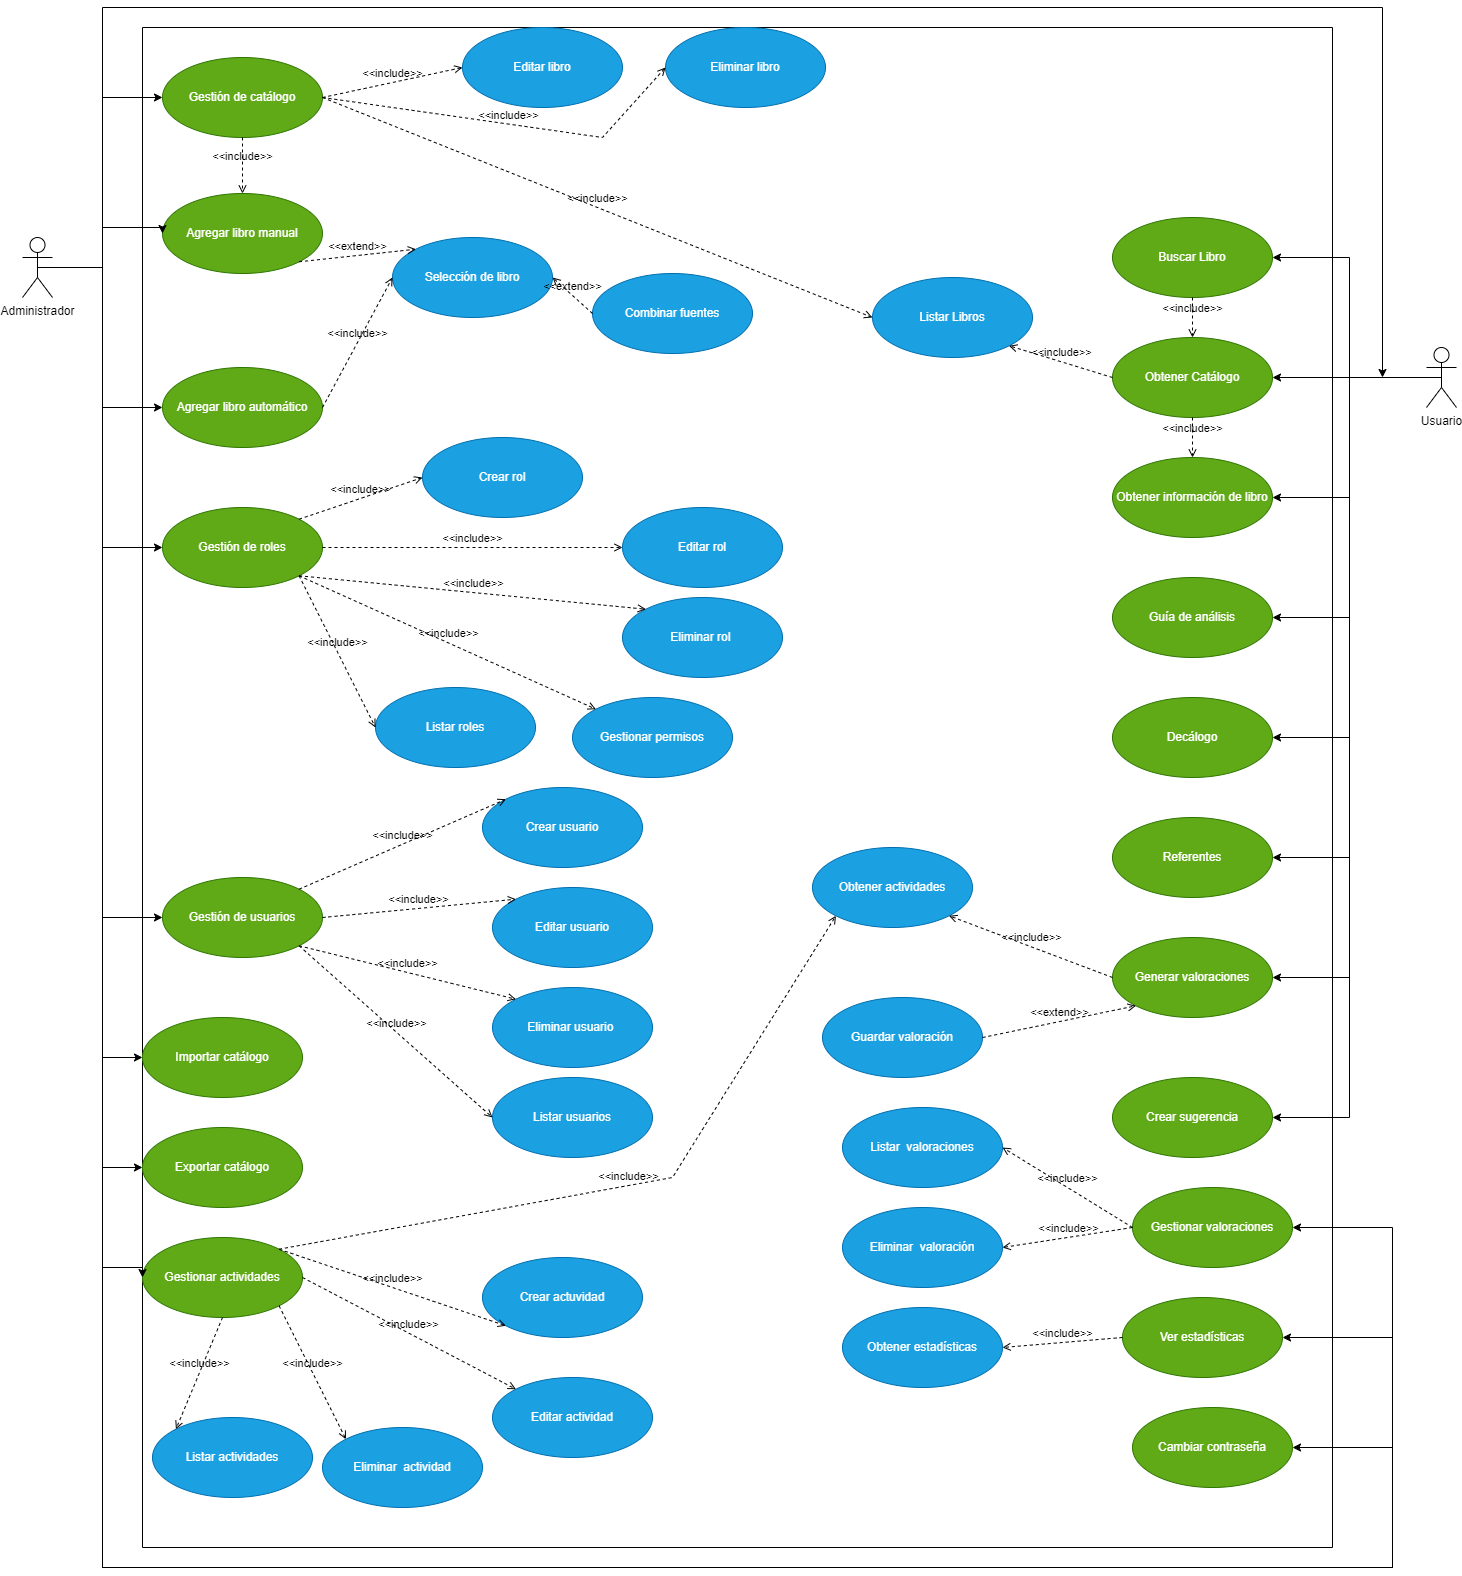
\includegraphics[width=\linewidth]{Imagenes/Diagrama de casos de uso.drawio.png}
    \caption{Diagrama de casos de uso}
    \label{Diagrama de casos de uso}
\end{figure}
\FloatBarrier
En esta sección, se presentan los diferentes casos de uso del proyecto. Cada caso de uso describe una secuencia de interacciones entre un usuario/a y el sistema, con el objetivo de alcanzar un resultado específico.
\begin{table}[p]
        \centering
        \begin{tabularx}{\linewidth}{ p{0.21\columnwidth} p{0.71\columnwidth} }
            \toprule
            \textbf{CU-1} & \textbf{Gestión de catálogo}\\
            \toprule
            \textbf{Versión} & 1.0 \\
            \textbf{Autor} & Daniel Fernández Fernández \\
            \textbf{Roles} & Administrador \\
            \textbf{Requisitos asociados} & RF-1.1, RF-1.2, RF-1.3, RF-1.4 \\
            \textbf{Descripción} & Permitir a la persona con rol de administración gestionar el catálogo de libros. \\
            \textbf{Precondición} & El administrador debe haber iniciado sesión. \\
            \textbf{Acciones} &
            \begin{enumerate}
            \def\labelenumi{\arabic{enumi}.}
            \tightlist
            \item El administrador selecciona Gestionar catálogo en el menú principal.
            \item El sistema muestra la lista completa de libros.
            \item El sistema muestra las opciones de edición, eliminación o más información de cada libro.
            \item El administrador realiza la acción deseada.
            \item El sistema guarda los cambios y actualiza el catálogo.
            \end{enumerate}\\
            \textbf{Postcondición} & El catálogo se actualiza con la acción realizada. \\
            \textbf{Excepciones} & El sistema muestra un mensaje de error si la acción no puede completarse. \\
            \textbf{Importancia} & Alta \\
            \bottomrule
        \end{tabularx}
        \caption{CU-1 Gestión de catálogo.}
\end{table}

\begin{table}[p]
        \centering
        \begin{tabularx}{\linewidth}{ p{0.21\columnwidth} p{0.71\columnwidth} }
            \toprule
            \textbf{CU-2} & \textbf{Agregar libro manual}\\
            \toprule
            \textbf{Versión} & 1.0 \\
            \textbf{Autor} & Daniel Fernández Fernández \\
            \textbf{Roles} & Administrador \\
            \textbf{Requisitos asociados} & RF-2.1 \\
            \textbf{Descripción} & Permitir a la persona con rol de administración agregar nuevos libros al catálogo de forma manual. \\
            \textbf{Precondición} & El administrador debe haber iniciado sesión. \\
            \textbf{Acciones} &
            \begin{enumerate}
            \def\labelenumi{\arabic{enumi}.}
            \tightlist
            \item El administrador selecciona Agregar libro manual en el menú.
            \item El sistema muestra un formulario para agregar un nuevo libro.
            \item El administrador completa el formulario con la información del libro.
            \item El administrador envía el formulario.
            \item El sistema guarda el nuevo libro en el catálogo.
            \end{enumerate}\\
            \textbf{Postcondición} & El libro nuevo se agrega al catálogo. \\
            \textbf{Excepciones} & El sistema no deja agregar si faltan datos obligatorios. \\
            \textbf{Importancia} & Alta \\
            \bottomrule
        \end{tabularx}
        \caption{CU-2 Agregar libro manual.}
\end{table}

\begin{table}[p]
        \centering
        \begin{tabularx}{\linewidth}{ p{0.21\columnwidth} p{0.71\columnwidth} }
            \toprule
            \textbf{CU-3} & \textbf{Agregar libro automático}\\
            \toprule
            \textbf{Versión} & 1.0 \\
            \textbf{Autor} & Daniel Fernández Fernández \\
            \textbf{Roles} & Administrador \\
            \textbf{Requisitos asociados} & RF-3.1, RF-3.2 \\
            \textbf{Descripción} & Permitir a la persona con rol de administración agregar libros al catálogo de forma automática desde diversas fuentes. \\
            \textbf{Precondición} & El administrador debe haber iniciado sesión. \\
            \textbf{Acciones} &
            \begin{enumerate}
            \def\labelenumi{\arabic{enumi}.}
            \tightlist
            \item El administrador selecciona Agregar libro automáticamente en el menú.
            \item El sistema muestra opciones de fuentes de datos disponibles.
            \item El administrador selecciona la fuente de datos o la combinación de los mismos.
            \item El sistema genera un formulario de los datos de los libros con las fuentes seleccionadas.
            \item El sistema agrega el libro generado al catálogo.
            \end{enumerate}\\
            \textbf{Postcondición} & Los libros nuevos se agregan al catálogo. \\
            \textbf{Excepciones} & El sistema muestra un mensaje de error si no se pueden obtener datos de las fuentes. \\
            \textbf{Importancia} & Media \\
            \bottomrule
        \end{tabularx}
        \caption{CU-3 Agregar libro automático.}
\end{table}

\begin{table}[p]
        \centering
        \begin{tabularx}{\linewidth}{ p{0.21\columnwidth} p{0.71\columnwidth} }
            \toprule
            \textbf{CU-4} & \textbf{Gestión de roles}\\
            \toprule
            \textbf{Versión} & 1.0 \\
            \textbf{Autor} & Daniel Fernández Fernández \\
            \textbf{Roles} & Administrador \\
            \textbf{Requisitos asociados} & RF-4.1, RF-4.2, RF-4.3, RF-4.4, RF-4.5 \\
            \textbf{Descripción} & Permitir a la persona con rol de administración gestionar los roles de usuario y sus permisos. \\
            \textbf{Precondición} & El administrador debe haber iniciado sesión. \\
            \textbf{Acciones} &
            \begin{enumerate}
            \def\labelenumi{\arabic{enumi}.}
            \tightlist
            \item El administrador selecciona Gestión de roles en el menú.
            \item El sistema muestra la lista de roles existentes.
            \item El administrador selecciona la opción de crear, editar, eliminar o modificar permisos de un rol.
            \item El sistema muestra el formulario correspondiente.
            \item El administrador completa el formulario y guarda los cambios.
            \end{enumerate}\\
            \textbf{Postcondición} & Los cambios en los roles se actualizan en el sistema. \\
            \textbf{Excepciones} & El sistema muestra un mensaje de error si la acción no puede completarse. \\
            \textbf{Importancia} & Alta \\
            \bottomrule
        \end{tabularx}
        \caption{CU-4 Gestión de roles.}
\end{table}

\begin{table}[p]
        \centering
        \begin{tabularx}{\linewidth}{ p{0.21\columnwidth} p{0.71\columnwidth} }
            \toprule
            \textbf{CU-5} & \textbf{Gestión de usuarios}\\
            \toprule
            \textbf{Versión} & 1.0 \\
            \textbf{Autor} & Daniel Fernández Fernández \\
            \textbf{Roles} & Administrador \\
            \textbf{Requisitos asociados} & RF-5.1, RF-5.2, RF-5.3, RF-5.4 \\
            \textbf{Descripción} & Permitir a la persona con rol de administración gestionar los usuarios del sistema. \\
            \textbf{Precondición} & El administrador debe haber iniciado sesión. \\
            \textbf{Acciones} &
            \begin{enumerate}
            \def\labelenumi{\arabic{enumi}.}
            \tightlist
            \item El administrador selecciona Gestión de usuarios en el menú.
            \item El sistema muestra la lista de usuarios existentes.
            \item El administrador selecciona la opción de crear, editar o eliminar un usuario.
            \item El sistema muestra el formulario correspondiente.
            \item El administrador completa el formulario y guarda los cambios.
            \end{enumerate}\\
            \textbf{Postcondición} & Los cambios en los usuarios se actualizan en el sistema. \\
            \textbf{Excepciones} & El sistema muestra un mensaje de error si la acción no puede completarse. \\
            \textbf{Importancia} & Alta \\
            \bottomrule
        \end{tabularx}
        \caption{CU-5 Gestión de usuarios.}
\end{table}

\begin{table}[p]
        \centering
        \begin{tabularx}{\linewidth}{ p{0.21\columnwidth} p{0.71\columnwidth} }
            \toprule
            \textbf{CU-5.5} & \textbf{Cambiar contraseña}\\
            \toprule
            \textbf{Versión} & 1.0 \\
            \textbf{Autor} & Daniel Fernández Fernández \\
            \textbf{Roles} & Administrador \\
            \textbf{Requisitos asociados} & RF-5.5 \\
            \textbf{Descripción} & Permitir a los usuarios registrados cambiar su contraseña. \\
            \textbf{Precondición} & El usuario debe haber iniciado sesión. \\
            \textbf{Acciones} &
            \begin{enumerate}
            \def\labelenumi{\arabic{enumi}.}
            \tightlist
            \item El usuario selecciona Cambiar contraseña en el menú.
            \item El sistema muestra un formulario para cambiar la contraseña.
            \item El usuario ingresa la nueva contraseña y la confirma.
            \item El usuario envía el formulario.
            \item El sistema actualiza la contraseña del usuario en la base de datos.
            \end{enumerate}\\
            \textbf{Postcondición} & La contraseña del usuario se actualiza correctamente. \\
            \textbf{Excepciones} & El sistema muestra un mensaje de error si la contraseña antigua no es correcta. \\
            \textbf{Importancia} & Alta \\
            \bottomrule
        \end{tabularx}
        \caption{CU-5.5 Cambiar contraseña.}
\end{table}

\begin{table}[p]
        \centering
        \begin{tabularx}{\linewidth}{ p{0.21\columnwidth} p{0.71\columnwidth} }
            \toprule
            \textbf{CU-6} & \textbf{Importar catálogo}\\
            \toprule
            \textbf{Versión} & 1.0 \\
            \textbf{Autor} & Daniel Fernández Fernández \\
            \textbf{Roles} & Administrador \\
            \textbf{Requisitos asociados} & RF-6.1 \\
            \textbf{Descripción} & Permitir a la persona con rol de administración importar un catálogo de libros desde un archivo externo. \\
            \textbf{Precondición} & El administrador debe haber iniciado sesión. \\
            \textbf{Acciones} &
            \begin{enumerate}
            \def\labelenumi{\arabic{enumi}.}
            \tightlist
            \item El administrador selecciona Importar en el menú.
            \item El sistema muestra una advertencia de seguridad.
            \item El sistema muestra una interfaz para seleccionar el archivo de importación.
            \item El administrador selecciona el archivo y confirma la importación.
            \item El sistema procesa el archivo y agrega los libros al catálogo.
            \end{enumerate}\\
            \textbf{Postcondición} & Los libros del archivo se agregan al catálogo. \\
            \textbf{Excepciones} & El sistema muestra un mensaje de error si no se puede procesar. \\
            \textbf{Importancia} & Media \\
            \bottomrule
        \end{tabularx}
        \caption{CU-6 Importar catálogo.}
\end{table}

\begin{table}[p]
        \centering
        \begin{tabularx}{\linewidth}{ p{0.21\columnwidth} p{0.71\columnwidth} }
            \toprule
            \textbf{CU-7} & \textbf{Exportar catálogo}\\
            \toprule
            \textbf{Versión} & 1.0 \\
            \textbf{Autor} & Daniel Fernández Fernández \\
            \textbf{Roles} & Administrador \\
            \textbf{Requisitos asociados} & RF-7.1 \\
            \textbf{Descripción} & Permitir a la persona con rol de administración exportar el catálogo de libros a un archivo. \\
            \textbf{Precondición} & El administrador debe haber iniciado sesión. \\
            \textbf{Acciones} &
            \begin{enumerate}
            \def\labelenumi{\arabic{enumi}.}
            \tightlist
            \item El administrador selecciona Exportar en el menú.
            \item El sistema muestra una interfaz para seleccionar el formato de exportación.
            \item El administrador selecciona el formato y confirma la exportación.
            \item El sistema genera el archivo y lo pone disponible para descarga.
            \end{enumerate}\\
            \textbf{Postcondición} & El archivo exportado está disponible para descarga. \\
            \textbf{Excepciones} & El sistema muestra un mensaje de error si la exportación falla. \\
            \textbf{Importancia} & Media \\
            \bottomrule
        \end{tabularx}
        \caption{CU-7 Exportar catálogo.}
\end{table}

\begin{table}[p]
        \centering
        \begin{tabularx}{\linewidth}{ p{0.21\columnwidth} p{0.71\columnwidth} }
            \toprule
            \textbf{CU-8} & \textbf{Gestionar actividades}\\
            \toprule
            \textbf{Versión} & 1.0 \\
            \textbf{Autor} & Daniel Fernández Fernández \\
            \textbf{Roles} & Administrador \\
            \textbf{Requisitos asociados} & RF-8.1, RF-8.2, RF-8.3, RF-8.4 \\
            \textbf{Descripción} & Permitir a la persona con rol de administración gestionar las actividades de las estimaciones. \\
            \textbf{Precondición} & El administrador debe haber iniciado sesión. \\
            \textbf{Acciones} &
            \begin{enumerate}
            \def\labelenumi{\arabic{enumi}.}
            \tightlist
            \item El administrador selecciona Gestión de actividades en el menú.
            \item El sistema muestra la lista de actividades existentes.
            \item El administrador selecciona la opción de crear, editar o eliminar una actividad.
            \item El sistema muestra el formulario correspondiente.
            \item El administrador completa el formulario y guarda los cambios.
            \end{enumerate}\\
            \textbf{Postcondición} & Los cambios en las actividades se actualizan en el sistema. \\
            \textbf{Excepciones} & El sistema muestra un mensaje de error si la acción no puede completarse. \\
            \textbf{Importancia} & Media \\
            \bottomrule
        \end{tabularx}
        \caption{CU-8 Gestionar actividades.}
\end{table}

\begin{table}[p]
        \centering
        \begin{tabularx}{\linewidth}{ p{0.21\columnwidth} p{0.71\columnwidth} }
            \toprule
            \textbf{CU-8.5} & \textbf{Obtener actividades}\\
            \toprule
            \textbf{Versión} & 1.0 \\
            \textbf{Autor} & Daniel Fernández Fernández \\
            \textbf{Roles} & Administrador y usuarios \\
            \textbf{Requisitos asociados} & RF-8.5 \\
            \textbf{Descripción} & Permitir a los usuarios obtener la lista de actividades disponibles en el apartado de valoración. \\
            \textbf{Precondición} & El usuario debe encontrarse en el valorador. \\
            \textbf{Acciones} &
            \begin{enumerate}
            \def\labelenumi{\arabic{enumi}.}
            \tightlist
            \item El usuario selecciona despliega los selectores de actividades en el valorador.
            \item El sistema muestra la lista de actividades disponibles.
            \end{enumerate}\\
            \textbf{Postcondición} & El usuario ve la lista de actividades disponibles. \\
            \textbf{Excepciones} & El sistema no muestra ninguna actividad en la lista. \\
            \textbf{Importancia} & Media \\
            \bottomrule
        \end{tabularx}
        \caption{CU-8.5 Obtener actividades.}
\end{table}


\begin{table}[p]
        \centering
        \begin{tabularx}{\linewidth}{ p{0.21\columnwidth} p{0.71\columnwidth} }
            \toprule
            \textbf{CU-9} & \textbf{Iniciar sesión}\\
            \toprule
            \textbf{Versión} & 1.0 \\
            \textbf{Autor} & Daniel Fernández Fernández \\
            \textbf{Roles} & Administrador \\
            \textbf{Requisitos asociados} & RF-9.1 \\
            \textbf{Descripción} & Permitir a los usuarios autenticarse en el sistema para acceder a sus funcionalidades. \\
            \textbf{Precondición} & El usuario debe estar registrado en el sistema. \\
            \textbf{Acciones} &
            \begin{enumerate}
            \def\labelenumi{\arabic{enumi}.}
            \tightlist
            \item El usuario selecciona Iniciar sesión en la página principal.
            \item El sistema muestra el formulario de inicio de sesión.
            \item El usuario ingresa su nombre de usuario y contraseña.
            \item El usuario envía el formulario.
            \item El sistema verifica las credenciales y autentica al usuario.
            \end{enumerate}\\
            \textbf{Postcondición} & El usuario autenticado puede acceder a las funcionalidades del sistema. \\
            \textbf{Excepciones} & El sistema muestra un mensaje de error si las credenciales son incorrectas. \\
            \textbf{Importancia} & Alta \\
            \bottomrule
        \end{tabularx}
        \caption{CU-9 Iniciar sesión.}
\end{table}

\begin{table}[p]
        \centering
        \begin{tabularx}{\linewidth}{ p{0.21\columnwidth} p{0.71\columnwidth} }
            \toprule
            \textbf{CU-10} & \textbf{Buscar libro}\\
            \toprule
            \textbf{Versión} & 1.0 \\
            \textbf{Autor} & Daniel Fernández Fernández \\
            \textbf{Roles} & Administrador y usuarios \\
            \textbf{Requisitos asociados} & RF-10.1 \\
            \textbf{Descripción} & Permitir a los usuarios buscar libros específicos en el catálogo. \\
            \textbf{Precondición} & El usuario debe estar en la página principal del catálogo o en la de inicio. \\
            \textbf{Acciones} &
            \begin{enumerate}
            \def\labelenumi{\arabic{enumi}.}
            \tightlist
            \item El usuario ingresa un término de búsqueda en el campo de búsqueda.
            \item El usuario envía la búsqueda.
            \item El sistema procesa la búsqueda y muestra los resultados correspondientes.
            \end{enumerate}\\
            \textbf{Postcondición} & El usuario ve los resultados de la búsqueda. \\
            \textbf{Excepciones} & El sistema muestra el catálogo vacío si no encuentra resultados. \\
            \textbf{Importancia} & Alta \\
            \bottomrule
        \end{tabularx}
        \caption{CU-10 Buscar libro.}
\end{table}

\begin{table}[p]
        \centering
        \begin{tabularx}{\linewidth}{ p{0.21\columnwidth} p{0.71\columnwidth} }
            \toprule
            \textbf{CU-11} & \textbf{Obtener catálogo}\\
            \toprule
            \textbf{Versión} & 1.0 \\
            \textbf{Autor} & Daniel Fernández Fernández \\
            \textbf{Roles} & Administrador y usuarios \\
            \textbf{Requisitos asociados} & RF-11.1 \\
            \textbf{Descripción} & Permitir a los usuarios obtener el catálogo completo de libros. \\
            \textbf{Precondición} & El usuario debe estar en la página principal del catálogo. \\
            \textbf{Acciones} &
            \begin{enumerate}
            \def\labelenumi{\arabic{enumi}.}
            \tightlist
            \item El usuario selecciona Catálogo en el menú.
            \item El sistema muestra la lista completa de libros disponibles.
            \end{enumerate}\\
            \textbf{Postcondición} & El usuario ve la lista completa de libros. \\
            \textbf{Excepciones} & El sistema muestra un mensaje si no hay libros disponibles. \\
            \textbf{Importancia} & Alta \\
            \bottomrule
        \end{tabularx}
        \caption{CU-11 Obtener catálogo.}
\end{table}


\begin{table}[p]
        \centering
        \begin{tabularx}{\linewidth}{ p{0.21\columnwidth} p{0.71\columnwidth} }
            \toprule
            \textbf{CU-12} & \textbf{Obtener información de libro}\\
            \toprule
            \textbf{Versión} & 1.0 \\
            \textbf{Autor} & Daniel Fernández Fernández \\
            \textbf{Roles} & Administrador y usuarios \\
            \textbf{Requisitos asociados} & RF-12.1 \\
            \textbf{Descripción} & Permitir a los usuarios ver la información detallada de un libro específico. \\
            \textbf{Precondición} & El usuario debe estar en la página del catálogo. El administrador puede acceder desde el gestor del catálogo \\
            \textbf{Acciones} &
            \begin{enumerate}
            \def\labelenumi{\arabic{enumi}.}
            \tightlist
            \item El usuario selecciona un libro de la lista.
            \item El sistema muestra la información detallada del libro seleccionado.
            \end{enumerate}\\
            \textbf{Postcondición} & El usuario ve la información detallada del libro. \\
            \textbf{Importancia} & Alta \\
            \bottomrule
        \end{tabularx}
        \caption{CU-12 Obtener información de libro.}
\end{table}



\begin{table}[p]
\centering
        \begin{tabularx}{\linewidth}{ p{0.21\columnwidth} p{0.71\columnwidth} }
            \toprule
            \textbf{CU-13} & \textbf{Gestionar valoraciones}\\
            \toprule
            \textbf{Versión} & 1.0 \\
            \textbf{Autor} & Daniel Fernández Fernández \\
            \textbf{Roles} & Administrador \\
            \textbf{Requisitos asociados} & RF-13.1, RF-13.2 \\
            \textbf{Descripción} & Mostrar una lista de valoraciones realizadas por los usuarios y sus acciones. \\
            \textbf{Precondición} & El usuario debe haber iniciado sesión. \\
            \textbf{Acciones} &
            \begin{enumerate}
            \def\labelenumi{\arabic{enumi}.}
            \tightlist
            \item El administrador selecciona valoraciones guardadas en el menú.
            \item El sistema muestra la lista de valoraciones disponibles.
            \item El administrador puede borrar valoraciones.
            \end{enumerate}\\
            \textbf{Postcondición} & El usuario ve la lista de valoraciones realizadas actualizada. \\
            \textbf{Excepciones} & El sistema muestra un listado vacío o un mensaje de error si no borra correctamente. \\
            \textbf{Importancia} & Media \\
            \bottomrule
        \end{tabularx}
        \caption{CU-13 Gestionar valoraciones.}
\end{table}


\begin{table}[p]
        \centering
        \begin{tabularx}{\linewidth}{ p{0.21\columnwidth} p{0.71\columnwidth} }
            \toprule
            \textbf{CU-14} & \textbf{Obtener estadísticas}\\
            \toprule
            \textbf{Versión} & 1.0 \\
            \textbf{Autor} & Daniel Fernández Fernández \\
            \textbf{Roles} & Administrador \\
            \textbf{Requisitos asociados} & RF-14.1 \\
            \textbf{Descripción} & Permitir a los usuarios obtener estadísticas relacionadas con la actividad y el catálogo. \\
            \textbf{Precondición} & El usuario debe haber iniciado sesión. \\
            \textbf{Acciones} &
            \begin{enumerate}
            \def\labelenumi{\arabic{enumi}.}
            \tightlist
            \item El administrador debe de encontrarse en el panel de administrador.
            \item El sistema muestra las estadísticas calculadas.
            \end{enumerate}\\
            \textbf{Postcondición} & El usuario ve las estadísticas relacionadas con la actividad y el catálogo. \\
            \textbf{Excepciones} & El sistema muestra unos gráficos vacíos si no se pueden obtener las estadísticas. \\
            \textbf{Importancia} & Media \\
            \bottomrule
        \end{tabularx}
        \caption{CU-14 Obtener estadísticas.}
\end{table}


\begin{table}[p]
        \centering
        \begin{tabularx}{\linewidth}{ p{0.21\columnwidth} p{0.71\columnwidth} }
            \toprule
            \textbf{CU-15} & \textbf{Generar valoraciones}\\
            \toprule
            \textbf{Versión} & 1.0 \\
            \textbf{Autor} & Daniel Fernández Fernández \\
            \textbf{Roles} & Administrador y usuarios \\
            \textbf{Requisitos asociados} & RF-15.1 \\
            \textbf{Descripción} & Permitir la generación de valoraciones basadas en parámetros definidos. \\
            \textbf{Precondición} & El usuario debe de encontrarse en valoraciones. \\
            \textbf{Acciones} &
            \begin{enumerate}
            \def\labelenumi{\arabic{enumi}.}
            \tightlist
            \item El usuario selecciona valoraciones en el menú.
            \item El sistema muestra una interfaz para definir los parámetros de la valoración.
            \item El usuario ingresa los parámetros y confirma la generación.
            \item El sistema genera las valoraciones basadas en los parámetros introducidos.
            \end{enumerate}\\
            \textbf{Postcondición} & Las valoraciones generadas calculan y se muestran. \\
            \textbf{Excepciones} & El sistema muestra un mensaje de error si la valoración falla. \\
            \textbf{Importancia} & Media \\
            \bottomrule
        \end{tabularx}
        \caption{CU-15 Generar valoraciones.}
\end{table}


\begin{table}[p]
        \centering
        \begin{tabularx}{\linewidth}{ p{0.21\columnwidth} p{0.71\columnwidth} }
            \toprule
            \textbf{CU-16} & \textbf{Crear sugerencia}\\
            \toprule
            \textbf{Versión} & 1.0 \\
            \textbf{Autor} & Daniel Fernández Fernández \\
            \textbf{Roles} & Administrador y usuarios \\
            \textbf{Requisitos asociados} & RF-16.1 \\
            \textbf{Descripción} & Permitir a los usuarios enviar sugerencias sobre libros. \\
            \textbf{Precondición} & El usuario debe estar en el catálogo. \\
            \textbf{Acciones} &
            \begin{enumerate}
            \def\labelenumi{\arabic{enumi}.}
            \tightlist
            \item El usuario selecciona el botón de sugerencia en el menú.
            \item El sistema muestra un formulario para ingresar la sugerencia.
            \item El usuario completa el formulario y envía la sugerencia.
            \item El sistema manda la sugerencia por correo al personal de administración.
            \end{enumerate}\\
            \textbf{Postcondición} & La sugerencia se envía correctamente. \\
            \textbf{Excepciones} & El sistema muestra un mensaje de error si la sugerencia no puede ser enviada. \\
            \textbf{Importancia} & Media \\
            \bottomrule
        \end{tabularx}
        \caption{CU-16 Crear sugerencia.}
\end{table}

